\documentclass[11pt]{article}
\usepackage{deauthor,times,graphicx}
%\usepackage[font=small,labelfont=bf]{caption}
\usepackage{caption}

\newcommand{\tfdv}{{\sf TFDV}}
\newcommand{\tfma}{{\sf TFMA}}
\newcommand{\extract}{{\sf tfma.Extract}}
\newcommand{\evaluation}{{\sf tfma.evaluators.Evaluation}}


\begin{document}

\title{Validating Data and Models in Continuous ML pipelines}
\author{ Mike Dreves, Gene Huang, Zhuo Peng, Neoklis Polyzotis, Evan Rosen, Paul Suganthan G. C.\\
{\small Google Inc.}}
\maketitle

\begin{abstract}
Production ML is more than writing the code for the trainer. It requires processes and tooling that enable a larger team to 
share, track, analyze, and monitor not only the code for ML but also the artifacts (Datasets, Models, ...) that are manipulated and 
generated in these production ML pipelines. 

In this paper we describe the tools we developed at Google for the analysis and validation of two of the most important types
of artifacts: Datasets and Models. These tools are currently deployed in production at Google and other large organizations. 
Our approach is heavily inspired by well-known principles of data-management systems. Ultimately, 
we want to enable users to trust their data and models, and understand how data properties affect the quality of the generated ML models. 
\end{abstract}

\section{Introduction}
ML has succeeded in tackling a wide range of challenging problems in practice, from medical applications (e.g., the detection of retinopathy~\cite{retinopathy}), to self-driving cars, or agriculture~\cite{cucumbers}, to name a few cases. Moreover, there is a fast pace of innovation in the scientific field of ML.

When one begins to use ML, they naturally think about writing the code that can train a model based on input data. This is an important step of using ML, but this code is only a small piece of what it takes to run ML reliably. In a production setting, the user of ML has to worry about: whether the input data has errors; how to trigger a retraining of the model when new data arrives; whether the new version of a model is good enough to replace the model currently used by the downstream stack; whether the serving data (used for prediction requests to the model) is sufficiently different such that retraining is required; and many more issues. 

At Google, we refer to this set of concerns as "ML engineering" in order to separate them from "ML coding", which refers to the relatively smaller task of writing the trainer. In using this term we draw an analogy to the distinction between software engineering and coding. Usually, coding refers to a one-off, monolithic piece of code that is not meant for sharing, whereas software engineering establishes processes and practices around versioning, testing, and so on, to enable a larger team to work on a shared code base that solves a bigger problem. The same applies to ML engineering: we need processes and tooling around versioning, testing,  monitoring, and so on, that apply not only to code but also to ML artifacts such as datasets and models. 

In this paper, we describe the tooling and processes we developed for the analysis and validation of datasets and models. These are two of the most important artifacts in production ML pipelines, with clear connections to the overall effectiveness of ML. We adopt a data-oriented approach to the management of these artifacts. This is obvious for dataset artifacts. For model artifacts, we note that the quality of a model is inherently tied to the data used for training, evaluation, and serving. Moreover, with the advent and maturation of Auto-ML solutions which can optimize the parameters of the model's architecture, the input data becomes the next obvious knob that can be tweaked to improve model quality. Thus, an approach based on data-management principles can be usefully extended to models.

Our work is in the context of TensorFlow Extended (TFX), a production-ML platform that we developed for Google's product teams and the world. The design and functionality of our tools is heavily influenced by our experience with ML in Google's production setting, but we believe that the basic principles and lessons learned apply to other contexts, and are of interest to both researchers and practitioners. 

\section{Data Validation}
ML crucially depends on the quality of the input data in order to produce a good model. In many cases, even simple errors in the data can affect significantly the resulting model. For example, consider a model that depends on an input data feature ``Country'' where the USA is represented with the string ``US''. However, if in the next batch of training data the value becomes ``USA'', then without any validation or pre-processing, the model will simply think that this is a new country.

Furthermore, it is often the case that the predictions from the generated models are logged and used to generate more data for training. Such feedback loops can amplify even ``small'' data errors and lead to gradual regression of model performance over a period of time. Hence, it is critical to catch data errors early, before they propagate through the complex loops and taint more of the pipeline's state.

Finally, error-free data is also critical for model understanding, since any attempt to debug and understand the output of the model or any quality metrics (e.g., AUC, precision, ...) is futile if the evaluation data has errors. All these observations indicate that we need to treat data as a first-class citizen in ML pipelines, on par with algorithms and infrastructure, with corresponding tooling to analyze, validate and monitor the data throughout the various stages of the pipeline.

Data validation is neither a new problem nor unique to ML, and so we can leverage techniques and principles from the field of data management. However, we argue that the problem acquires unique characteristics in the context of ML and hence we need to rethink existing solutions. First, we need a way to express ML-related constraints and expectations on the quality of the data. Second, the data validation system must generate reliable alerts with high precision, and provide enough context for the human to quickly identify the root cause of the problem. This is due to the fact that in most cases data errors cannot be fixed automatically -- they require some human intervention, either in the ML pipeline (e.g., rolling back the trainer to a checkpoint unaffected by the suspect data) or in the data-generation code (e.g., fixing the bugs that cause the errors). Third, the system needs to scale to production pipelines which typically process billions to trillions of examples. Finally, the system needs to account for the fact that data is stored and managed externally from the ML pipeline, and often in a variety of storage systems, and hence a-priori knowledge about the data and its semantics is limited.

To address the above challenges in the context of Google's production ML pipelines, we developed TensorFlow Data Validation (\tfdv) \cite{tfdvdemo, tfdvsysml, tfdv}, a scalable data analysis and validation system for ML. Our system is deployed in production as an integral part of TFX~\cite{tfx}, an end-to-end ML platform, and is used by hundreds of product teams at Google to monitor and validate trillions of training and serving examples per day, amounting to several petabytes of data per day. We recently open sourced \tfdv\ and the system has received significant attention from the open-source community as well: more than 50M downloads since the first release in October 2018, plus it has influenced the development of other open-source data validation systems such as Apache Spark Data Validation~\footnote{https://databricks.com/session/apache-spark-data-validation}. Furthermore, \tfdv\ has been adopted by other large organizations using ML, e.g., see Spotify's keynote at TensorFlow World 2019 about using \tfdv\ \footnote{https://www.youtube.com/watch?v=zxd3Q2gdArY\&t=748s}.

Few recent works (\cite{datavalidationamazon}, \cite{failingloudly}) have considered the importance of data validation for ML applications. For example,  Amazon (Schelter et. al. \cite{datavalidationamazon}) proposed a system for automating data quality verification task that provides a declarative API to specify common quality constraints and custom validation code. While Amazon’s system allows users to express arbitrary constraints, we opted to have a restrictive schema definition language that captures the data constraints for most of our users in order to focus on reliable high precision alerts. Further, our work emphasizes the user-mediated co-evolution of the schema with data and the model. As far as we can tell, TFDV is the first open-source data analysis and validation system for ML.

\begin{figure}[t]
  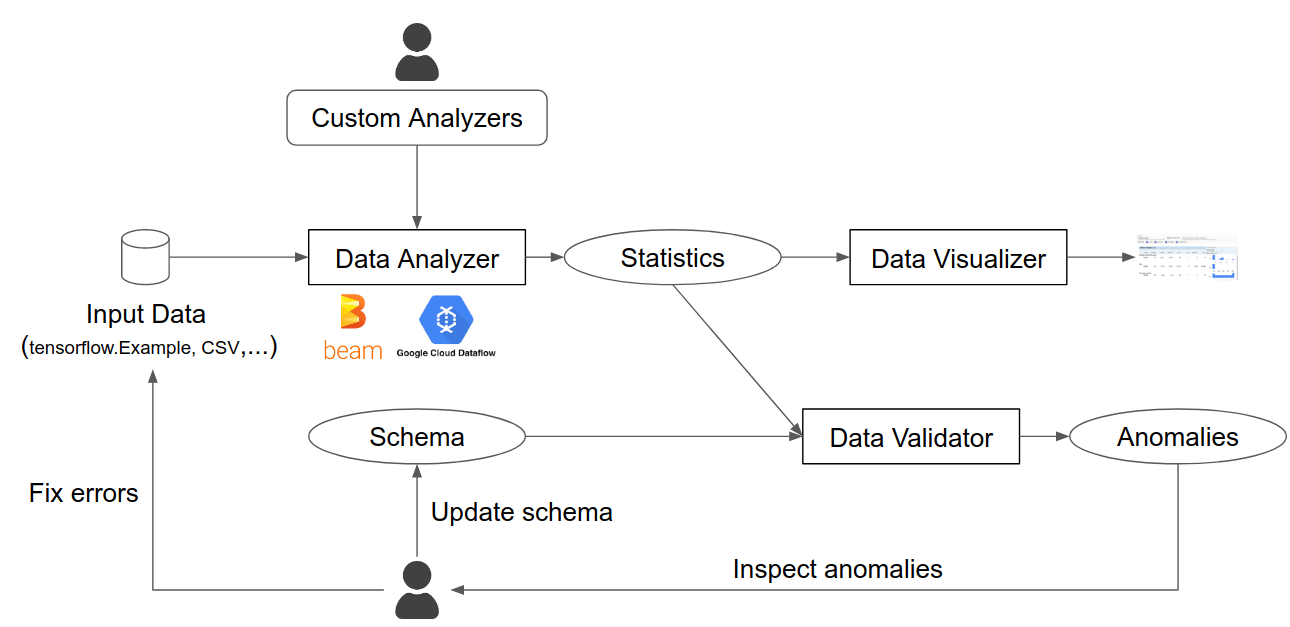
\includegraphics[width=\linewidth]{submissions/continuous-pipelines/figs/arch2.png}
  \caption{TensorFlow Data Validation Architecture.}
  \label{arch}
\vspace{-4mm}
\end{figure}

\subsection{System Overview}
Figure 1 shows the \tfdv\ architecture which consists of a Data Analyzer component which computes statistics in a scalable fashion over large amounts of data, a Data Validator which finds anomalies in the data, and a Data Visualizer which provides visualizations of the statistics, schema, and the anomalies.

\paragraph{Data Analyzer.} Data Analyzer takes a collection of statistics generators and computes data statistics needed for validation. \tfdv\ uses Apache Beam \cite{beam} to define and process its data pipelines. The statistics generators are implemented as Beam transforms. Users can provide custom statistics generators which are executed together with the default generators.
The generator API takes Apache Arrow Tables as input, as it is powerful enough to encode popular logical training data formats: flat (tensorflow.Example, CSV), sequence (tensorflow.SequenceExample) or structured data (e.g. Protocol Buffers or Apache Avro). \tfdv\  provides decoders for popular data formats like tensorflow.Example, and CSV. Users can write custom decoders (that convert their input to Arrow Tables) to handle arbitrary data formats. Realizing the data pipelines using Beam allows \tfdv\ to transparently run the pipeline in different environments such as a single machine, Flink/Spark cluster, and Google Cloud Dataflow.

The statistics computed by \tfdv\ include individual feature statistics depending on the type of the feature (e.g., statistics such as min, max, mean, median, histogram etc. for numeric features, statistics such as number of unique values, top-k values, average length etc. for categorical features.) and cross-feature statistics (e.g., correlation between features and mutual information of a feature with the label etc.). We represent the statistics as a protocol buffer message (See \cite{tfmd} for the complete list of statistics computed by \tfdv.).

\paragraph{Data Validator.} The Data Validator checks the properties of the data as specified through a schema. Typically we expect the data characteristics to remain stable across different splits of data (e.g., training data and evaluation data) or batches of data that are close in time. Hence, we consider any deviation within a batch (or split) from the expected data characteristics as an $anomaly$.

\tfdv\ adapts the “battle-tested” principles from data management systems to the context of ML. Specifically, in order to codify these expected data characteristics, \tfdv\ generalizes the traditional notion of a $schema$ from database systems. The schema follows a logical data model where each training or serving example is a collection of features, with each feature having several constraints attached to it. This flat model has an obvious mapping to the flat data formats such as tensorflow.Example or CSV. The constraints associated with each feature cover some basic properties (e.g., type, domain, valency) but also constraints that are relevant to ML (See \cite{tfdvsysml} for a more detailed discussion of our schema formalism.). Using a schema also allows us to verify any assumptions of training/serving code (e.g., the schema can be used to generate fuzzy examples and verify if the training/serving code crashes on those examples) and thereby catch potential model crashes early on. We represent the schema as a protocol buffer message.

\tfdv\ supports two types of validation: (1) validating a single batch of data against the schema, and (2) validating two batches of data (e.g., are there any significant changes between training and serving data, or between successive batches of the training data?). Any disagreement found during validation is flagged as an anomaly for human inspection and further investigation. See \cite{tfdv} for the complete list of 52 anomalies identified by \tfdv\ and the conditions on which each anomaly is raised.

\paragraph{Data Visualizer.} \tfdv\ provides visualizations for the statistics, schema and the anomalies. It provides a simple table-based view for the schema and the anomalies. It uses the Facets library \cite{facets} to visualize the statistics (see Figure \ref{stats}). Specifically, \tfdv\ supports (1) visualizing the statistics of a batch of data, and (2) comparing statistics between batches of data.

\begin{figure}[t]
  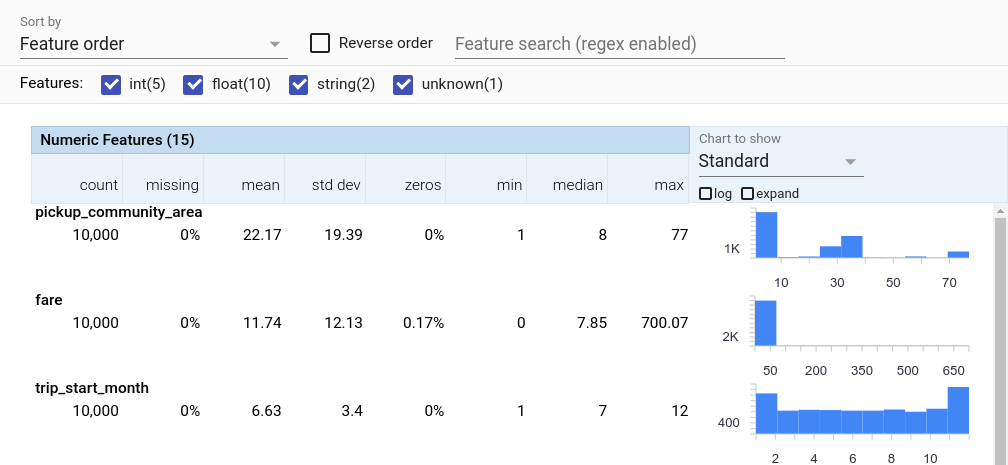
\includegraphics[width=\linewidth]{submissions/continuous-pipelines/figs/stats1.png}
  \caption{Exploring data using Facets visualization.}
  \label{stats}
\vspace{-4mm}
\end{figure}

\begin{figure}[t]
  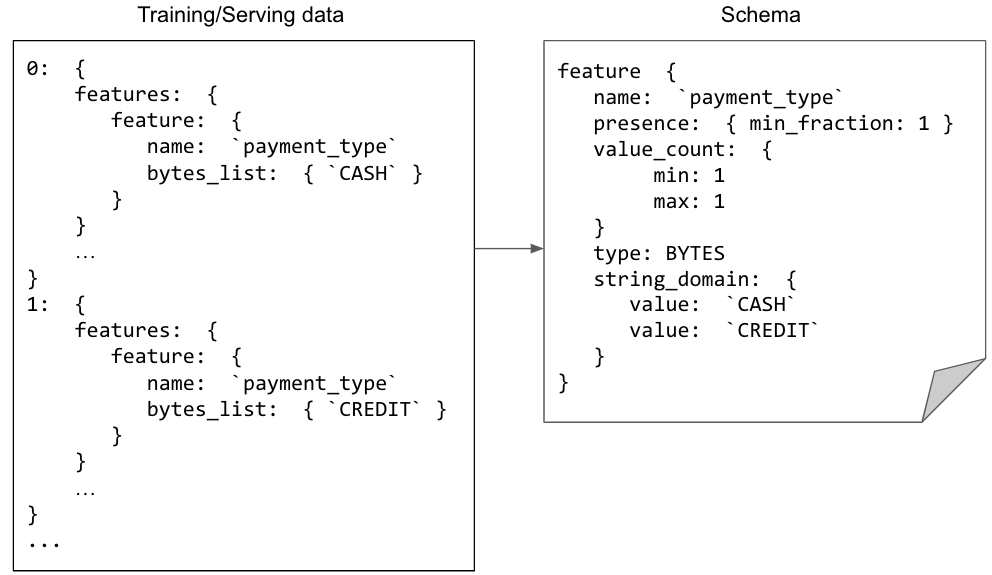
\includegraphics[width=\linewidth]{submissions/continuous-pipelines/figs/schemainfer1.png}
  \caption{An example schema and corresponding data in the tf.train.Example format.}
  \label{schema}
\vspace{-4mm}
\end{figure}

\newpage
\subsection{Inferring an initial schema} As described in Section 2.1, \tfdv\ uses a schema to capture the stable data characteristics. Our assumption
is that the users are responsible to curate the schema. However, many ML pipelines use thousands of features, and so constructing a schema manually for such pipelines can be quite tedious. Furthermore, the domain knowledge of the features may be distributed across a number of engineers within the product team or
even outside of the team. In such cases, the upfront effort in schema construction can discourage engineers from setting up data validation until they run into a serious data error.

To overcome this adoption hurdle, \tfdv\ provides a way to auto-generate the initial schema. This auto-generated schema attempts to capture salient properties of the data without overfitting to a particular batch of data. Avoiding overfitting is important: an overfitted schema is more likely to cause spurious alerts when validating a new batch of data, which in turn increases the cognitive overhead for the on-call engineers, reduces their trust in the system, and may even lead them to switch off data validation altogether. We currently rely on a set of reasonable heuristics to perform this initial schema inference. A more formal solution, perhaps with guarantees or controls on the amount of overfitting, is an interesting direction for future work. We assume the user will inspect the inferred schema and modify any properties if needed. Figure \ref{schema} shows a sample schema. The schema is represented as a protocol buffer.

\subsection{Performing skew detection}
Training/Serving skew refers to a difference in the feature values or distributions between the data used to train a model and the data observed by the serving system. \tfdv\ allows users to check if there are significant changes between training and serving data. \tfdv\ supports skew detection based on $L_{\infty}$ distance \cite{tfdvsysml} and Jensen–Shannon divergence \cite{jsd}.


\section{Model Validation}

After training a model based on (validated) input data, the next step in a production pipeline is analyzing the trained model and deciding whether it can be pushed to the inference/serving stack. This step makes the model available to other applications. However, pushing a model that returns sub-optimal or even erroneous predictions can lead to undesired downstream effects. As an example, if a bad model generates uninteresting or irrelevant recommendations in a movie-streaming service the user experience is likely to suffer. What is needed is the equivalent of an integration test, where we can evaluate the model's accuracy on unseen data. For this purpose, we have developed TensorFlow Model Analysis (\tfma)~\cite{tfma}, a scalable model evaluation system. Similar to \tfdv\, \tfma\ is deployed in production as an integral part of TFX platform and is used by hundreds of product teams at Google to evaluate ML models. \tfma\ was open sourced in March 2018 and has received significant attention from the open-source community (more than 50M downloads).

While data validation prevents errors through inappropriate input data, it is still possible to introduce errors into the pipeline as a result of improper training. Most ML frameworks provide tools for evaluating metrics of interest (e.g., loss or AUC) during training. \tfma\ takes this a step further by allowing users to re-evaluate their models post-training over large amounts of data in a distributed manner (using Apache Beam). This evaluation can be done using the same metrics that were defined during training or with additional metrics added after the model has been generated. While \tfma\ performs full passes over generally much larger data than is seen at training time, the datasets are still just samples drawn from a larger population. To help gauge the reliability of these computations, \tfma\ provides confidence intervals for the metrics it computes. For increased reliability and safety, \tfma\ provides a means to set expectations on model performance metrics using either absolute thresholds or thresholds relative to a baseline. Practitioners can then gate pushing their models to production based on passing the said validation thresholds. In a sense, this model-based validation complements the data-based validation implemented by \tfdv.

\tfma\ also supports computing and validating model metrics on data slices. Model metrics computed on the whole evaluation dataset can mask interesting or significant deviations of the same metrics computed on data slices that correspond to meaningful sub-populations. For instance, a machine-translation model may perform adequately well on average but significantly worse on a specific language. \tfma\ allows users to declare slices of interest and then to get a more detailed view of model metrics computed on the corresponding subsets of the evaluation data. Model validation can subsequently verify these metrics in order to guard against model regressions which only affect a small but important slice of the evaluation data.

\begin{figure}[t]
  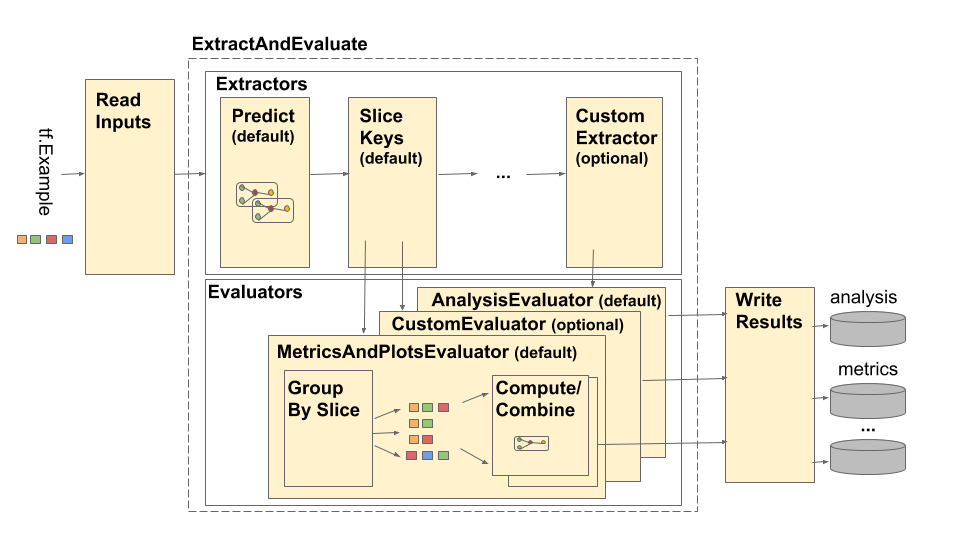
\includegraphics[width=\linewidth]{submissions/continuous-pipelines/figs/tfma_pipeline.png}
  \caption{TensorFlow Model Analysis Architecture.}
  \label{tfmaarch}
\vspace{-4mm}
\end{figure}

\subsection{System Overview}
Figure \ref{tfmaarch} shows the \tfma\ architecture which consists of four components: 1) Reading the inputs, 2) Extraction, 3) Evaluation, and 4) Writing results. These components make use of two primary types: \extract\ and \evaluation. The type \extract\ represents the data that is extracted during pipeline processing whereas the type \evaluation\ represents the output from evaluating the extracts at various points during the pipeline. In order to provide a flexible API, these types are just Python dictionaries where the keys are defined (reserved for use) by different implementations.  

\paragraph{Extraction.} The extraction process is a list of Beam transforms that are run in series. The extractors take \extract\ as input and return \extract\ as output. For example, PredictExtractor is one of the default extractors which uses the input extract produced by the read inputs transform and runs it through a model to produce extracts that contains the predictions. \tfma\ allows users to provide custom extractors that can be inserted at any point in the extraction process.

\paragraph{Evaluation.} Evaluation is the process of taking an extract and evaluating it. An evaluator is a Beam transform that takes \extract\ as inputs and outputs \evaluation. \tfma\ supports a wide variety of model metrics and plots as documented in \cite{tfmametrics}, which are computed as part of the evaluation process. For example, the default MetricsAndPlotsEvaluator uses the features, labels, and predictions in the extracts as input, group the extracts by slices, and then performs metrics and plots computations. Further, users can also provide custom evaluators. \tfma\ provides visualizations for the metrics and plots as shown in Figure \ref{tfmaui}.

\begin{figure}[t]
  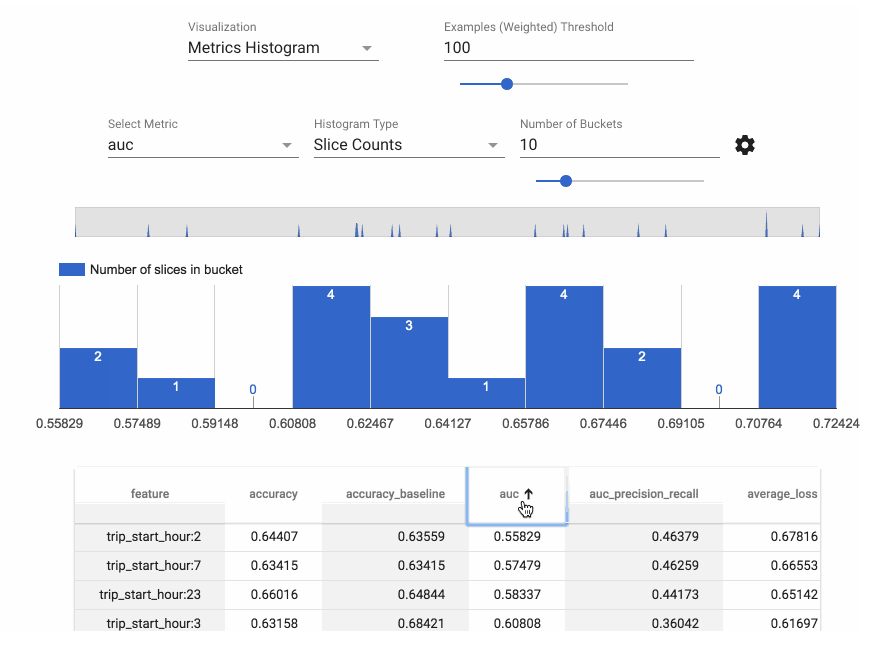
\includegraphics[width=\linewidth]{submissions/continuous-pipelines/figs/tfma_ui.png}
  \caption{Visualization of sliced model metrics.}
  \label{tfmaui}
\vspace{-4mm}
\end{figure}


\subsection{Automatically Identifying Problematic Slices}
As mentioned in Section 3, \tfma\ can compute model metrics over slices of data that are of interest to the user. For example, Figure \ref{tfmaui} shows the model metrics sliced by ``trip\_start\_hour" feature. However in many cases, users do not know a priori which slices are important. Alternatively, a user might miss important sub-slices within the manually defined slices (e.g., the machine-translation model may under-perform for a specific language only when the translation request comes from a specific class of devices). To aid with these cases we investigated techniques to automatically identify slices of interest~\cite{slicefinder}. We view this automatic slicing as a complement to the manual slicing already supported by \tfma. For instance, it is possible to start with manually defined slices and then automatically discover subslices of interest. Our inspiration in this domain has been previous works in discovering interesting roll-ups/drill-downs in data cubes~\cite{sarawagi2000user, sathe2001intelligent, 10.14778/2733004.2733035}. Moreover, recent work~\cite{NIPS2019_9137} in the ML community has shown how knowledge about under-performing slices can be leveraged in order to improve overall model quality.

\newpage
\section{Conclusion}
In this paper, we described the tools and processes developed at Google for the analysis and validation of two of the most important artifacts in an ML pipeline: $datasets$ and $models$. Specifically, we described \tfdv, a data validation system, and \tfma, a model evaluation system. The developed tools have been used extensively within Google and has received significant attention from the open-source community.  

\begin{thebibliography}{10}
\itemsep=1pt

\bibitem{retinopathy}
\newblock Diagnosing Diabetic Retinopathy with Machine Learning.
\newblock
  \url{https://about.google/intl/en\_us/stories/seeingpotential}

\bibitem{jsd}
\newblock Jensen–Shannon divergence.
\newblock
  \url{https://en.wikipedia.org/wiki/Jensen-Shannon\_divergence}
  
\bibitem{cucumbers}
\newblock How a Japanese cucumber farmer is using deep learning and TensorFlow.
\newblock
  \url{https://cloud.google.com/blog/products/gcp/how-a-japanese-cucumber-farmer-is-using-deep-learning-and-tensorflow}

\bibitem{tfma}
\newblock TensorFlow Model Analysis.
\newblock
  \url{https://www.tensorflow.org/tfx/model\_analysis/get\_started}

\bibitem{tfmametrics}
\newblock TensorFlow Model Analysis - Metrics and Plots.
\newblock
  \url{https://www.tensorflow.org/tfx/model\_analysis/metrics}

\bibitem{tfdv}
\newblock TensorFlow Data Validation.
\newblock
  \url{https://www.tensorflow.org/tfx/data\_validation/get\_started}

\bibitem{facets}
\newblock Facets.
\newblock
  \url{https://pair-code.github.io/facets/}

\bibitem{beam}
\newblock Apache Beam.
\newblock
  \url{https://beam.apache.org/}

\bibitem{tfmd}
\newblock TensorFlow Metadata.
\newblock
  \url{https://github.com/tensorflow/metadata}

\bibitem{tfx}
Denis Baylor, et al.
\newblock TFX: A TensorFlow-Based Production-Scale Machine Learning Platform.
\newblock In {\em ACM SIGKDD}, 2017.

\bibitem{slicefinder}
 Yeounoh Chung, et al.
\newblock Slice Finder: Automated Data Slicing for Model Validation.
\newblock In {\em IEEE ICDE}, pages 1550--1553, 2019.

\bibitem{tfdvsysml}
Eric Breck, et al.
\newblock Data Validation for Machine Learning.
\newblock In {\em SysML}, 2019.

\bibitem{tfdvdemo}
Emily Caveness, et al.
\newblock TensorFlow Data Validation: Data Analysis and Validation in Continuous ML Pipelines.
\newblock In {\em ACM SIGMOD Demo}, 2020.

\bibitem{sarawagi2000user}
Sunita Sarawagi.
\newblock User-adaptive exploration of multidimensional data.
\newblock In {\em VLDB}, volume~2000, pages 307--316, 2000.

\bibitem{sathe2001intelligent}
Gayatri Sathe, and Sunita Sarawagi.
\newblock Intelligent rollups in multidimensional OLAP data.
\newblock In {\em VLDB}, volume~1, pages 531--540, 2001.

\bibitem{NIPS2019_9137}
Vincent Chen, et al.
\newblock Slice-based Learning: A Programming Model for Residual Learning in Critical Data Slices.
\newblock In {\em Advances in Neural Information Processing Systems}, pages 9397--9407, 2019.

\bibitem{10.14778/2733004.2733035}
Manasi Vartak, et al..
\newblock SeeDB: Automatically Generating Query Visualizations.
\newblock In {\em PVLDB}, volume~7, number~13, pages 1581--1584, 2014.

\bibitem{failingloudly}
Rabanser, Stephan and G\"{u}nnemann, Stephan and Lipton, Zachary.
\newblock Failing Loudly: An Empirical Study of Methods for Detecting Dataset Shift.
\newblock In {\em Advances in Neural Information Processing Systems}, 2019.

\bibitem{datavalidationamazon}
Sebastian Schelter, et al.
\newblock Automating Large-Scale Data Quality Verification.
\newblock In {\em VLDB}, volume~11, number~12, pages 1781--1794, 2018.


\end{thebibliography}

\end{document}